%%%%%%%%%%%%%%%%%%%%%%%%%%%%%%%%%%%%%%%%%%%%%%%%
%% Compile the master file!
%% 		Slides: Antonio Machicao y Priemer
%% 		Course: Wissenschaftliches Arbeiten
%%%%%%%%%%%%%%%%%%%%%%%%%%%%%%%%%%%%%%%%%%%%%%%%


%%%%%%%%%%%%%%%%%%%%%%%%%%%%%%%%%%%%%%%%%%%%%%%%%%%%
%%%             Metadata                         
%%%%%%%%%%%%%%%%%%%%%%%%%%%%%%%%%%%%%%%%%%%%%%%%%%%%  

\title{
	\LaTeX\ for Linguists
}

\subtitle{\LaTeX\ 5: Linguistic packages 1}

\author[aMyP]{
	{\small Sebastian Nordhoff \& Antonio Machicao y Priemer}
	\\
	{\footnotesize \url{www.linguistik.hu-berlin.de/staff/amyp}}
	%	\\
	%	{\footnotesize \href{mailto:mapriema@hu-berlin.de}{mapriema@hu-berlin.de}}
}

\institute{LOT 2019, Amsterdam}

%\date{ }

%\publishers{\textbf{6. linguistischer Methodenworkshop \\ Humboldt-Universität zu Berlin}}

%\hyphenation{nobreak}


%%%%%%%%%%%%%%%%%%%%%%%%%%%%%%%%%%%%%%%%%%%%%%%%%%%%
%%%             Preamble's End                   
%%%%%%%%%%%%%%%%%%%%%%%%%%%%%%%%%%%%%%%%%%%%%%%%%%%%      


%%%%%%%%%%%%%%%%%%%%%%%%%%%%%%%%%%%
%%%%%%%%%%%%%%%%%%%%%%%%%%%%%%%%%%%    
%% Title slide 
\begin{frame}
  \HUtitle
\end{frame}


%% Contents slide
\frame{
%\begin{multicols}{2}
	\frametitle{Contents}
%	\tableofcontents[hideallsubsections]
	\tableofcontents
	%[pausesections]
%\end{multicols}
	}


%%%%%%%%%%%%%%%%%%%%%%%%%%%%%%%%%%%%
%%%%%%%%%%%%%%%%%%%%%%%%%%%%%%%%%%%%
%% Extra literature

\nocite{Freitag&MyP15a}
\nocite{Knuth1986}
\nocite{Kopka94a}
\nocite{MyP17c}
\nocite{MyP&Kerkhof16a}
	
%%%%%%%%%%%%%%%%%%%%%%%%%%%%%%%%%%%%
%%%%%%%%%%%%%%%%%%%%%%%%%%%%%%%%%%%%


%%%%%%%%%%%%%%%%%%%%%%%%%%%%%%%%%%%%%
%%%%%%%%%%%%%%%%%%%%%%%%%%%%%%%%%%%%%
%%%% Basic literature for these slides
%
%\begin{frame}
%\frametitle{Grundlage \& empfohlene Lektüre}
%
%\dots basierend auf \citet{Freitag&MyP15a} und auf \citet{MyP&Kerkhof16a}\\
%\ras \href{https://www.researchgate.net/publication/279514740_LATEX-Einfuhrung_fur_Linguisten}{LINK}
%
%
%\nocite{Kopka94a}
%
%\end{frame}


%%%%%%%%%%%%%%%%%%%%%%%%%%%%%%%%%%
%%%%%%%%%%%%%%%%%%%%%%%%%%%%%%%%%%
\section{Transcriptions with IPA}
\frame{
	\frametitle{~}
	%	\begin{multicols}{2}
	\tableofcontents[currentsection,hideallsubsections]
	%	\end{multicols}
}
%%%%%%%%%%%%%%%%%%%%%%%%%%%%%%%%%%
%%%%%%%%%%%%%%%%%%%%%%%%%%%%%%%%%%

\begin{frame}[fragile]
\frametitle{Transcriptions with IPA}

With Xe\LaTeX , you can use \textbf{Unicode characters} for your transcriptions:

\smallskip

You can copy the Unicode characters for transcriptions from here:\\
\url{http://ipa.typeit.org/full/}
%[ʔ ɛ t͡s ə n d ə ʁ ɐ]

\smallskip

Some fonts cannot display all Unicode characters, \fe try to copy the Unicode characters for the following word and compile using first \ltxpack{lmodern} and then \ltxpack{libertine}.

\ea \textipa{["PE\t{ts}@nd@\textscr{}5]}
\z 

\pause 

\bigskip

The package \textbf{\ltxpack{tipa}} offers commands for transcriptions with IPA, but it is not compatible with all other packages. %\fe with \ltxpack{libertine}

\begin{lstlisting}
\usepackage{tipa}
\end{lstlisting}

%\begin{itemize}
%	\item \ltxpack{tipa} definiert bestimmte \LaTeX -Befehle um. Abhängig von der Font-Kodierung sind manchmal zusätzliche Einstellungen nötig, bspw.\ die Optionen \ltxterm{T3} und \ltxterm{T1} (in dieser Reihenfolge) beim Paket \ltxpack{fontenc} und die Optionen \ltxterm{noenc} und \ltxterm{safe} beim Paket \ltxpack{tipa}.
%\end{itemize}

%\begin{lstlisting}
%\usepackage[T3,T1]{fontenc}
%
%\usepackage[noenc,safe]{tipa}	
%\end{lstlisting}

\end{frame}


%%%%%%%%%%%%%%%%%%%%%%%%%%%%%%%%%%
\begin{frame}[fragile]
%\frametitle{}

\ltxterm{tipa} provides 3 ways to use IPA characters:


\textbf{macros:}

\begin{lstlisting}
[\textglotstop{}an.\textesh{}\textinvscr{}\texttoptiebar{a\textsci{}}.
\textschwa{}n]

[\textsecstress\textepsilon kspl\textschwa \textprimstress ne\textsci\textesh
\textschwa n]
\end{lstlisting}

\vspace{-.25cm}

\begin{multicols}{2}
\ea {[\textglotstop{}an.\textesh{}\textinvscr{}\texttoptiebar{a\textsci{}}.\textschwa{}n]}

\ex {[\textsecstress\textepsilon kspl\textschwa \textprimstress ne\textsci\textesh\textschwa n]}
\z 
\end{multicols}


\textbf{groups of macros:}

\vspace{-.25cm}

\begin{multicols}{2}
\begin{lstlisting}
\textipa{[Pan.SK\t{aI}.@n]} 
\textipa{[""Ekspl@"neIS@n]}
\end{lstlisting}


\ea \textipa{[Pan.SK\t{aI}.@n]}

\ex \textipa{[""Ekspl@"neIS@n]}	
\z 	
\end{multicols}


\textbf{\ltxterm{tipa} environment:}

\vspace{-.25cm}

\begin{multicols}{2}
	
\begin{lstlisting}
\begin{IPA}
[Pan.SK\t{aI}.@n]

[""Ekspl@"neIS@n]
\end{IPA}
\end{lstlisting}


\ea	\begin{IPA}
[Pan.SK\t{aI}.@n]
\end{IPA}

\ex \begin{IPA} 
[""Ekspl@"neIS@n]
\end{IPA}
\z
\end{multicols}

\nocite{Rei04a}

\nocite{Linke05a}

\end{frame}


%%%%%%%%%%%%%%%%%%%%%%%%%%%%%%%%%%%
%\begin{frame}[fragile]
%%\frametitle{IPA-Notation}
%
%\begin{itemize}
%	\item Die IPA-Transkriptionen können in verschiedenen Schriftarten eingebettet werden:
%\end{itemize}
%
%{\scriptsize
%\begin{tabular}{lll}
%	aktuelle        & \lstinline|\textipa{Pan.SK\texttoptiebar{aI}.@n}|          & \textipa{Pan.SK\texttoptiebar{aI}.@n}          \\
%	Standardschrift &                                                            &                                                \\
%	Slanted         & \lstinline|\textsl{\textipa{Pan.SK\texttoptiebar{aI}.@n}}| & \textsl{\textipa{Pan.SK\texttoptiebar{aI}.@n}} \\
%	Bold            & \lstinline|\textbf{\textipa{Pan.SK\texttoptiebar{aI}.@n}}| & \textbf{\textipa{Pan.SK\texttoptiebar{aI}.@n}} \\
%	Sans Serif      & \lstinline|\textsf{\textipa{Pan.SK\texttoptiebar{aI}.@n}}| & \textsf{\textipa{Pan.SK\texttoptiebar{aI}.@n}} \\
%	Typewriter      & \lstinline|\texttt{\textipa{Pan.SK\texttoptiebar{aI}.@n}}| & \texttt{\textipa{Pan.SK\texttoptiebar{aI}.@n}} \\
%\end{tabular}
%}
%
%
%\end{frame}


%%%%%%%%%%%%%%%%%%%%%%%%%%%%%%%%%%%
%\begin{frame}[fragile]
%%\frametitle{IPA-Notation}
%
%\begin{itemize}
%\item Für weitere Features des \ltxpack{tipa}-Pakets schauen Sie sich die Dokumentation an: \citet{Rei04a}
%
%\item Eine gute Auflistung der benötigten Befehle für IPA-Transkriptionen mittels \ltxpack{tipa} finden Sie unter: \citet{Linke05a}
%\end{itemize}
%
%\end{frame}


%%%%%%%%%%%%%%%%%%%%%%%%%%%%%%%%%%
%%%%%%%%%%%%%%%%%%%%%%%%%%%%%%%%%%
\section{Verbatim }
\frame{
	\frametitle{~}
%	\begin{multicols}{2}
		\tableofcontents[currentsection, hideallsubsections]
%	\end{multicols}
}
%%%%%%%%%%%%%%%%%%%%%%%%%%%%%%%%%%

\begin{frame}[fragile]
\frametitle{Verbatim}

If you want to \textbf{write code}, \LaTeX\ provides the \textbf{\ltxterm{verb} command} and the \textbf{\ltxterm{verbatim} environment}.

\begin{multicols}{2}
	
\begin{lstlisting}
\verb|\textbf{test}|

\begin{verbatim}
\textbf{test}
\end{verbatim}

\end{lstlisting}	

\columnbreak

\verb|\textbf{test}|

\begin{verbatim}
\textbf{test}
\end{verbatim}

\end{multicols}

\end{frame}


%%%%%%%%%%%%%%%%%%%%%%%%%%%%%%%%%%
\begin{frame}[fragile]
%\frametitle{Bibliography database}

With the package \ltxpack{listings}, \textbf{more options} for verbatim can be specified:

\begin{lstlisting}
\usepackage{listings}

\lstset{
language=TeX,
backgroundcolor=\color{lightgray},
basicstyle={\footnotesize\ttfamily\color{blue}},
showstringspaces=false,
columns=flexible
}
\end{lstlisting}

\bigskip

This package offers an \textbf{in-line version} with the \lstinline|\lstinline| \textbf{command} 
and the \lstinline|lstlisting| \textbf{environment}.

\bigskip

For the in-line version, use \textbf{characters as delimiters} for your command \lstinline|\lstinline| that are not used in your code.



\end{frame}

%%%%%%%%%%%%%%%%%%%%%%%%%%%%%%%%%%
\begin{frame}[fragile]
%\frametitle{Bibliographiedatenbank}


Entries in your database have the following syntax:

%\begin{multicols}{2}

\begin{lstlisting}
@book{Knuth1986,
author = {Knuth, Donald E.},
address = {Boston, MA},
publisher = {Addison-Wesley},
title = {The TeXbook},
year = {1986}
}
\end{lstlisting}

%\columnbreak
%
%\end{multicols}

\begin{itemize}
	\item \lstinline|@book|: type of \textbf{reference}
	\item \lstinline|{ }|: \textbf{brackets} around the complete entry \lstinline|@book{ }|\\
	and around every single information segment \lstinline|author = { }|
	
	\item \lstinline|Knuth1986|: a unique \textbf{ID} for the entry
	\item \lstinline|,|: commas as separation for the information segments
	\item \lstinline|author| \lstinline|address| etc.: type of information provided
\end{itemize}

The single information segments have always the same syntax: \lstinline|type of information = {information},|

\smallskip 

Which information depends on the \textbf{reference type} and the \textbf{bibliography style}.
\end{frame}


%%%%%%%%%%%%%%%%%%%%%%%%%%%%%%%%%%%
%\begin{frame}[fragile]
%%\frametitle{Literaturangaben}
%
%\begin{itemize}
%\item Die Datenbank können Sie \textbf{mit jedem beliebigen Texteditor} bearbeiten. 
%
%\item Verwenden Sie \ltxpack{TeXstudio} für die Bearbeitung Ihrer \ltxterm{.bib}-Datei, werden die verschiedenen Teile besonders \textbf{hervorgehoben}.
%
%
%\end{itemize}
%
%\begin{figure}
%\centering
%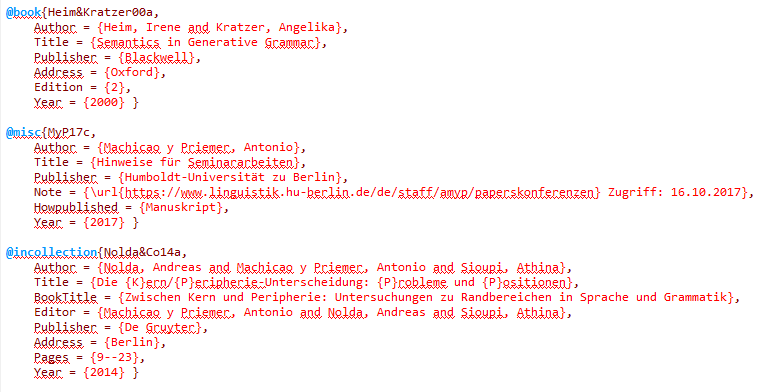
\includegraphics[width=.90\textwidth]{../../texfiles-beamer/tex-material/WissArb-latex/bibeintraege}
%\end{figure}
%
%\nocite{Heim&Kratzer00a}
%\nocite{MyP17c}
%\nocite{Nolda&Co14a}
%
%\end{frame}


%%%%%%%%%%%%%%%%%%%%%%%%%%%%%%%%%%%
%\begin{frame}[fragile]
%%\frametitle{Literaturangaben}
%
%\begin{itemize}
%
%\item Ist die Datei in \ltxpack{TeXstudio} offen, werden die IDs bei der \textbf{Autovervollständigung} angezeigt.
%\end{itemize}
%
%\begin{figure}
%\centering
%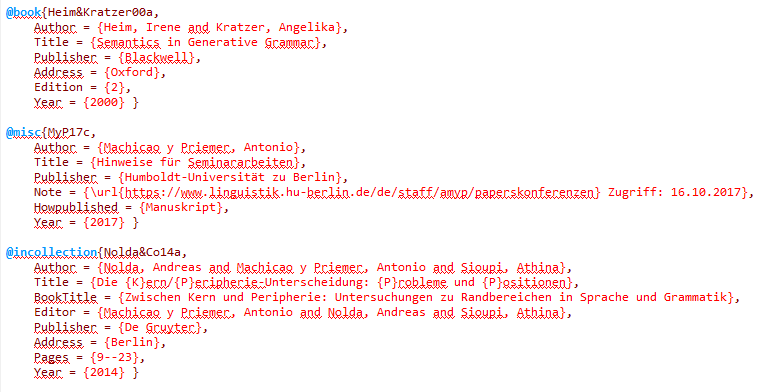
\includegraphics[width=.90\textwidth]{../../texfiles-beamer/tex-material/WissArb-latex/bibeintraege}
%\end{figure}
%
%\end{frame}


%%%%%%%%%%%%%%%%%%%%%%%%%%%%%%%%%%
\begin{frame}[fragile]
%\frametitle{Literaturangaben}


The most important \textbf{entry types} are:

\begin{enumerate}
\item \textbf{\ltxterm{article}} for articles in journals or magazines
\item \textbf{\ltxterm{book}} for published books
\item \textbf{\ltxterm{incollection}} for an article in a edited book
\item \textbf{\ltxterm{inproceedings}} for articles in conference proceedings
\item \textbf{\ltxterm{mastersthesis}} for master thesis (not in every style available)
\item \textbf{\ltxterm{phdthesis}} for dissertations
\item \textbf{\ltxterm{unpublished}} for documents with author and title but not published
\item \textbf{\ltxterm{misc}} the joker in case nothing else fits
\end{enumerate}

\pause 

\begin{itemize}

\item You can find a list of the \textbf{required} and \textbf{optional information segments} for every entry type in:\\
\url{https://en.wikipedia.org/wiki/BibTeX}

%\item Eine Liste der \textbf{obligatorischen} und \textbf{optionalen Informationspunkte} je nach Eintrag finden Sie hier:
%
%\url{https://de.wikipedia.org/wiki/BibTeX}

\item For further information on Bib\TeX :\\
\url{www.bibtex.org}
\end{itemize}

\end{frame}


%%%%%%%%%%%%%%%%%%%%%%%%%%%%%%%%%%
\begin{frame}[fragile]
%\frametitle{Literaturangaben}

\textbf{Examples of entry types:}

\bigskip


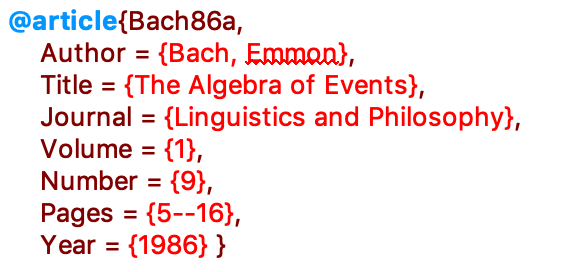
\includegraphics[scale=.5]{../../texfiles-beamer/tex-material/WissArb-latex/xelatex-bib-article}

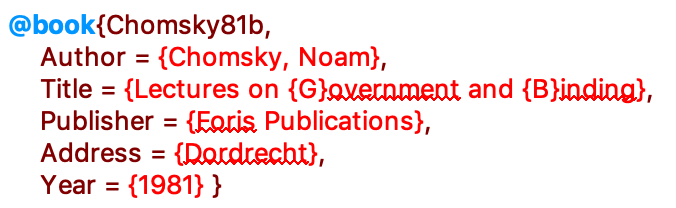
\includegraphics[scale=.5]{../../texfiles-beamer/tex-material/WissArb-latex/xelatex-bib-book}

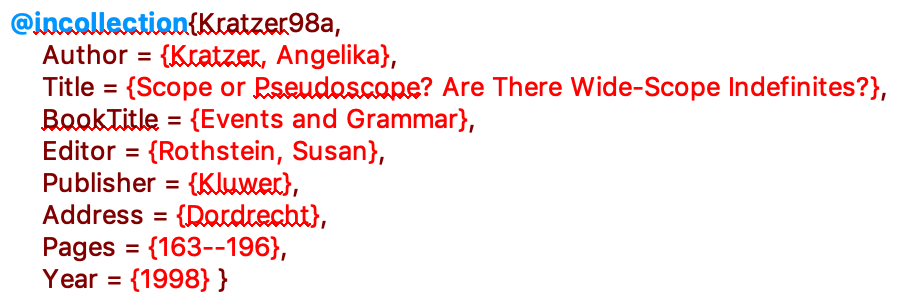
\includegraphics[scale=.5]{../../texfiles-beamer/tex-material/WissArb-latex/xelatex-bib-incollection}

\end{frame}

%%%%%%%%%%%%%%%%%%%%%%%%%%%%%%%%%%
%%%%%%%%%%%%%%%%%%%%%%%%%%%%%%%%%%
\section{Using your references}
\frame{
\frametitle{~}
%\begin{multicols}{2}
\tableofcontents[currentsection,hideallsubsections]
%\end{multicols}
}
%%%%%%%%%%%%%%%%%%%%%%%%%%%%%%%%%%

\begin{frame}[fragile]
\frametitle{Using your references}

Using your references is similar to using \ltxterm{ref}, but with the command \textbf{\ltxterm{cite}} (or versions of it) and the \textbf{ID} of the entry:

\begin{lstlisting}
\cite{ID}
\end{lstlisting}

%\vspace{.3cm}

If a reference should \textbf{appear in your bibliography}, but \textbf{not in your text}, then use \textbf{\ltxterm{nocite}} and the \textbf{ID}:

\begin{lstlisting}
\nocite{ID}
\end{lstlisting}

\pause 

\textbf{Example:}

\begin{lstlisting}
The following entry appear in the text and in the bibliography (cf.\ end of this 
presentation): \cite{Loebner15a}.
On the other hand, the following entry is not appearing in the text but in the 
bibliography (cf.\ end of this presentation): \nocite{ZimmermannT&Sternefeld13a}
\end{lstlisting}

\outputbox{
The following entry appear in the text and in the bibliography (cf.\ end of this 
presentation): \cite{Loebner15a}.

On the other hand, the following entry is not appearing in the text but in the 
bibliography (cf.\ end of this presentation): \nocite{ZimmermannT&Sternefeld13a}
}

\end{frame}


%%%%%%%%%%%%%%%%%%%%%%%%%%%%%%%%%%
%%%%%%%%%%%%%%%%%%%%%%%%%%%%%%%%%%
\section{Bibliography style \& bibliography}
\frame{
	\frametitle{~}
%	\begin{multicols}{2}
		\tableofcontents[currentsection,hideallsubsections]
%	\end{multicols}
}
%%%%%%%%%%%%%%%%%%%%%%%%%%%%%%%%%%

\begin{frame}[fragile]
\frametitle{Bibliography style \& bibliography}

\begin{itemize}
	\item The ways your \textbf{in-text citations} and your \textbf{bibliography} is formatted depends on your \textbf{bibliography style}. 
	
%	Das Aussehen des \textbf{Literaturverzeichnisses} und der im Fließtext angegebenen \textbf{Quellen} hängt vom \textbf{Bibliographiestil} ab.
	
	\item The following styles are always included (other styles are loaded for instance with packages):
	
	\begin{itemize}
		\item \ltxterm{alpha.bst}
		\item \ltxterm{abbrv.bst} (useful for abstracts)
		\item \ltxterm{plain.bst}
		\item \ltxterm{unsrt.bst}
	\end{itemize}

%	\item Die Stile sind \idR für das Englische geschrieben. Im Netz finden Sie andere Stile für das Deutsche.

\item At the position you want your bibliography to appear, put the following commands:

%Am \textbf{Ende des Dokuments} (oder an der \textbf{Position, an der die Literaturliste erscheinen soll}) wird die \textbf{Verlinkung zur eigenen Bibliographiedatenbank} erstellt. Das Literaturverzeichnis wird an dieser Stelle gedruckt.

%\item Es ist empfehlenswert den \textbf{Bibliographiestil} an der gleichen Stelle \textbf{festzulegen}.

\end{itemize}

\begin{multicols}{2}

\begin{lstlisting}
\bibliographystyle{name of style}
\bibliography{name of .bib-file} 
\end{lstlisting}

\columnbreak

\begin{lstlisting}
\bibliographystyle{langsci-unified}
\bibliography{myFirstBibliography} 
\end{lstlisting}

\end{multicols}

\end{frame}

%%%%%%%%%%%%%%%%%%%%%%%%%%%%%%%%%%
\begin{frame}[fragile]
\frametitle{Style: alpha}

\begin{figure}
\centering
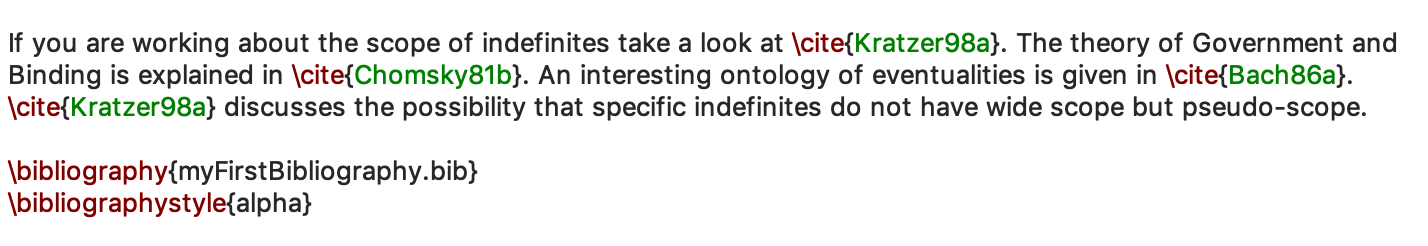
\includegraphics[width=.85\textwidth]{../../texfiles-beamer/tex-material/WissArb-latex/xelatex-bib-alpha}
\end{figure}

\begin{figure}
\centering
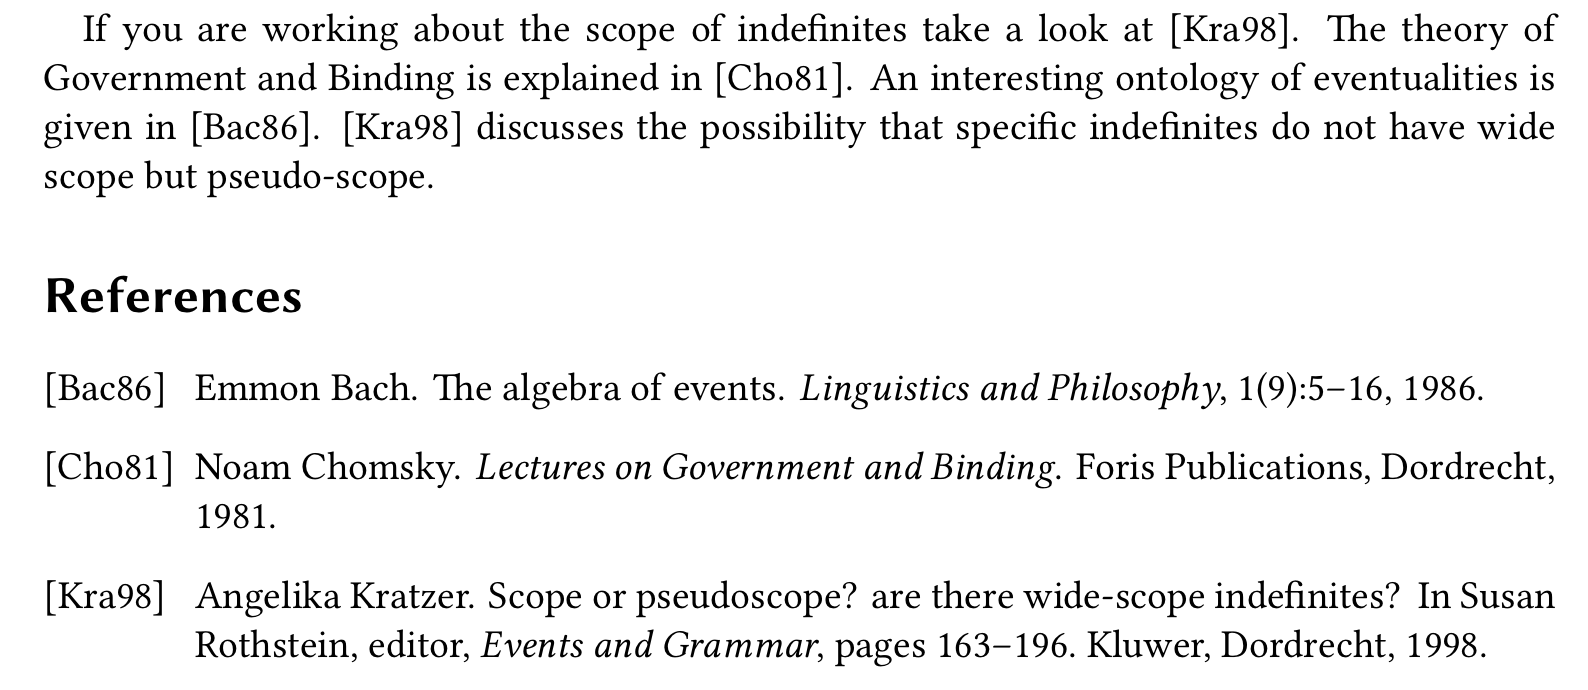
\includegraphics[width=.85\textwidth]{../../texfiles-beamer/tex-material/WissArb-latex/xelatex-bib-alpha-pdf}
\end{figure}

\end{frame}


%%%%%%%%%%%%%%%%%%%%%%%%%%%%%%%%%%
\begin{frame}[fragile]
\frametitle{Style: abbrv}

\begin{figure}
\centering
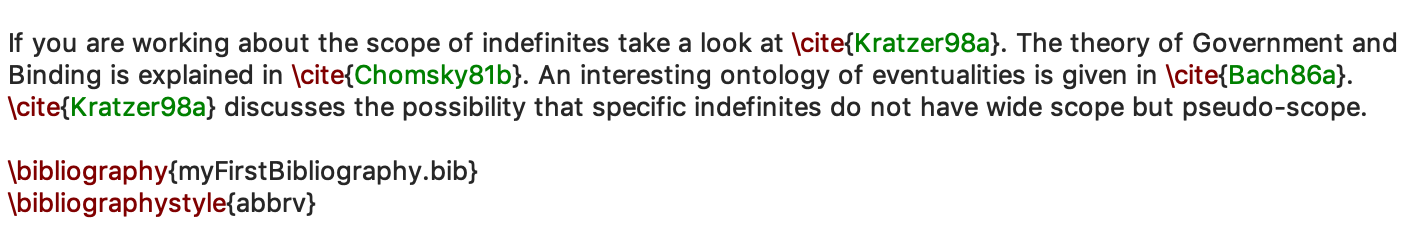
\includegraphics[width=.85\textwidth]{../../texfiles-beamer/tex-material/WissArb-latex/xelatex-bib-abbrv}
\end{figure}

\begin{figure}
\centering
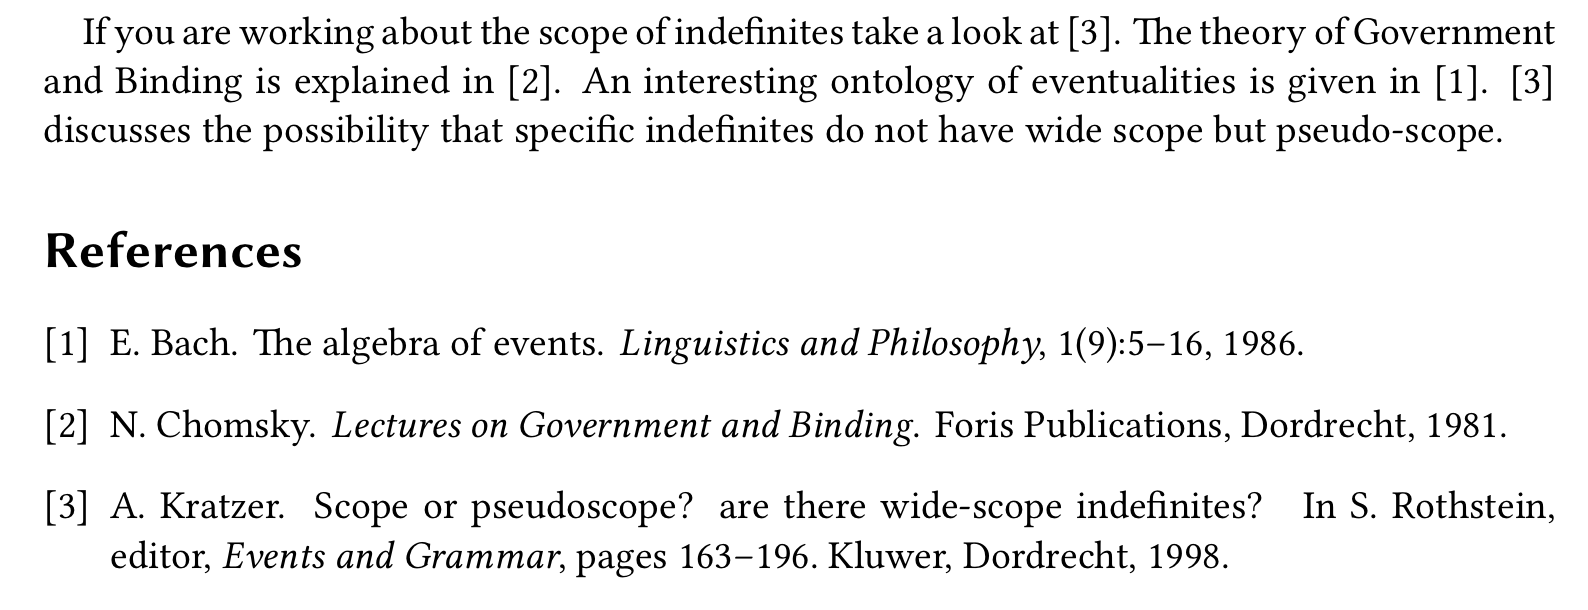
\includegraphics[width=.85\textwidth]{../../texfiles-beamer/tex-material/WissArb-latex/xelatex-bib-abbrv-pdf}
\end{figure}

\end{frame}


%%%%%%%%%%%%%%%%%%%%%%%%%%%%%%%%%%%
%\begin{frame}[fragile]
%\frametitle{Stil: plain}
%
%\begin{figure}
%\centering
%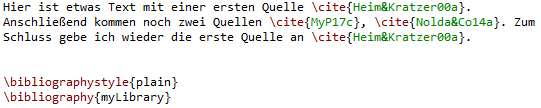
\includegraphics[width=.70\textwidth]{../../texfiles-beamer/tex-material/WissArb-latex/bib_plain_tex}
%\end{figure}
%
%\begin{figure}
%\centering
%
\includegraphics[width=.70\textwidth]{../../texfiles-beamer/tex-material/WissArb-latex/bib_plain_pdf}
%\end{figure}
%
%\end{frame}


%%%%%%%%%%%%%%%%%%%%%%%%%%%%%%%%%
%%%%%%%%%%%%%%%%%%%%%%%%%%%%%%%%%
\section{More citation commands}
\frame{
	\frametitle{~}
%	\begin{multicols}{2}
		\tableofcontents[currentsection,hideallsubsections]
%	\end{multicols}
}
%%%%%%%%%%%%%%%%%%%%%%%%%%%%%%%%%%

\begin{frame}[fragile]
\frametitle{More citation commands}

\begin{itemize}
	\item Besides \ltxterm{cite} and \ltxterm{nocite}, further commands for citations can be used. These commands can be loaded with packages, \fe \ltxpack{natbib} or \ltxpack{biblatex} with the option \ltxpack{natbib}. 
	
%	\item Um den in der Linguistik häufig benutzten \textbf{\ltxterm{author(year)}-Stil} zu verwenden, sollte das Paket mit dieser \textbf{Option} geladen werden:
	
\begin{lstlisting}
\usepackage[authoryear]{natbib}
\end{lstlisting}
	
	\item \ltxpack{natbib} offers \textbf{more bibliography styles}, \fe \ltxterm{chicago} and \ltxterm{apalike}, which are compatible with the \ltxterm{author(year)} notation used in linguistics.
	
\end{itemize}

\nocite{Daly10a}

%\end{frame}


%%%%%%%%%%%%%%%%%%%%%%%%%%%%%%%%%%%%
%\begin{frame}[fragile]
%
%\begin{itemize}
%\item Hier die in unserer Präambel geladenen Pakete bisher:
%\end{itemize}
%
%\begin{figure}
%\centering
%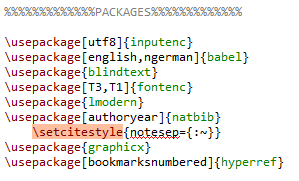
\includegraphics[width=.70\textwidth]{../../texfiles-beamer/tex-material/WissArb-latex/preamble3}
%\end{figure}
%
%
%\end{frame}


%%%%%%%%%%%%%%%%%%%%%%%%%%%%%%%%%%%
%\begin{frame}[fragile]

\textbf{Extra commands:}

\vspace{-.5cm}

\begin{multicols}{2}
%\small	

\begin{lstlisting}
\citet{Knuth1986}
\citet[36]{Knuth1986}
\citep{Knuth1986}
\citep[36]{Knuth1986}
\citep[cf.][36]{Knuth1986}
\citep[cf.][]{Knuth1986}
\end{lstlisting}

Knuth (1986)\\
Knuth (1986, 36)\\
%Knuth (vgl.\ 1986, 36)\\
(Knuth, 1986)\\
(Knuth, 1986, 36)\\
(cf.\ Knuth, 1986, 36)\\
(cf.\ Knuth, 1986)\\
%\citet{Knuth1986}\newline 
%\citet[36]{Knuth1986}\newline
%\citet[vgl.][36]{Knuth1986}\newline  % ?
%\citep{Knuth1986}\newline 
%\citep[36]{Knuth1986}\newline
%\citep[vgl.][36]{Knuth1986}\newline 
%\citep[vgl.][]{Knuth1986}\newline
\end{multicols}

%\pause

%\begin{itemize}
%\item Um zwischen Jahres- und Seitenzahl einen \textbf{Doppelpunkt statt eines Kommas} zu verwenden, können \textbf{Spezifikationen zum Stil} beim Laden des Pakets geladen werden: 
%\begin{lstlisting}
%\usepackage[authoryear]{natbib}
%\setcitestyle{notesep={:~}}
%\end{lstlisting}
%\end{itemize}

\end{frame}


%%%%%%%%%%%%%%%%%%%%%%%%%%%%%%%%%%%
\begin{frame}[fragile]
%\frametitle{Literaturangaben}


\begin{lstlisting}
\usepackage[authoryear]{natbib}
\setcitestyle{notesep={:~}}
\end{lstlisting}

\footnotesize

\begin{tabular}{lll}
\textbf{code}                               & \textbf{colon}            & \textbf{comma} \\

\lstinline|\citet{Knuth1986}|               & \citet{Knuth1986}               & Knuth (1986)   \\

\lstinline|\citet[36]{Knuth1986}|           & \citet[36]{Knuth1986}           & Knuth (1986, 36)   \\

\lstinline|\citet[cf.][36]{Knuth1986}| & \citet[cf.][36]{Knuth1986} & Knuth (cf.\ 1986, 36)  \\

\lstinline|\citep{Knuth1986}|               & \citep{Knuth1986}               & (Knuth, 1986)   \\

\lstinline|\citep[36]{Knuth1986}|     & \citep[36]{Knuth1986}           & (Knuth, 1986, 36) \\

\lstinline|\citep[cf.][36]{Knuth1986}|       & \citep[cf.][36]{Knuth1986}     & (cf.\ Knuth, 1986, 36)   \\

\lstinline|\citep[cf.][]{Knuth1986}|           & \citep[cf.][]{Knuth1986}       & (cf.\ Knuth, 1986)
\end{tabular}

%\end{frame}
%
%
%%%%%%%%%%%%%%%%%%%%%%%%%%%%%%%%%%%
%\begin{frame}[fragile]
%%\frametitle{Literaturangaben}

\pause 

\bigskip

Commands for citations \textbf{without brackets}:

\begin{multicols}{2}
\begin{lstlisting}
\citealt{Knuth1986}
\citealp{Knuth1986}
\end{lstlisting}
\citealt{Knuth1986}\newline
\citealp{Knuth1986}
\end{multicols}

\pause 

Commands for citations of \textbf{part of the information}:

%\noindent Hier einige Beispiele um nur \textbf{Teile der Information} zu erhalten:

\begin{multicols}{2}
\begin{lstlisting}
\citeauthor{Knuth1986}
\citeyear{Knuth1986}
\citeyearpar{Knuth1986}
\end{lstlisting}
\citeauthor{Knuth1986}\newline
\citeyear{Knuth1986}\newline
\citeyearpar{Knuth1986}
\end{multicols}

\end{frame}


%%%%%%%%%%%%%%%%%%%%%%%%%%%%%%%%%%%
%\begin{frame}[fragile]
%%\frametitle{Literaturangaben}
%
%\noindent Diese Befehle können bspw.\ verwendet werden, um Verweise in Genitiv zu setzen:
%
%\begin{lstlisting}
%\dots\ wie in 
%\citeauthor{Knuth1986}s \citeyearpar{Knuth1986}
%Buch bereits gesehen \dots\
%\end{lstlisting}
%\outputbox{
%\dots\ wie in 
%\citeauthor{Knuth1986}s \citeyearpar{Knuth1986}
%Buch bereits gesehen \dots\ 
%}
%
%\end{frame}


%%%%%%%%%%%%%%%%%%%%%%%%%%%%%%%%%%
\begin{frame}[fragile]
%\frametitle{Literaturangaben}

Citing \textbf{more than one reference} with one command:

\begin{lstlisting}
\citep[cf.][]{Knuth1986,Rothstein11a,Meindl11a}.
\end{lstlisting}

\outputbox{
\citep[cf.][]{Knuth1986,Rothstein11a,Meindl11a}.
}
\vspace{1em}


\pause 

More than two names are \textbf{abbreviated with ``et al.''} in the citation:

\begin{lstlisting}
\citet{Nolda&Co14a} vs. \citet{Pollard&Sag94a}
\end{lstlisting}

\outputbox{
\citet{Nolda&Co14a} vs. \citet{Pollard&Sag94a}
}

\end{frame}



%%%%%%%%%%%%%%%%%%%%%%%%%%%%%%%%%%
\begin{frame}[fragile]
\frametitle{Style: chicago}


\begin{figure}
\centering
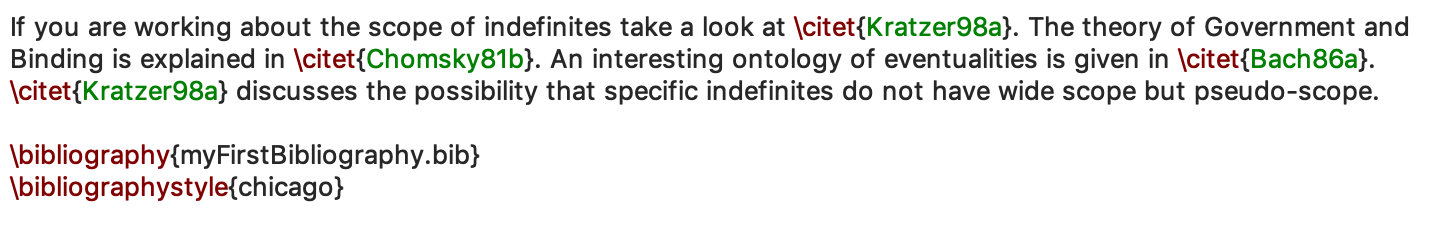
\includegraphics[width=.85\textwidth]{../../texfiles-beamer/tex-material/WissArb-latex/xelatex-bib-chicago}
\end{figure}

\begin{figure}
\centering
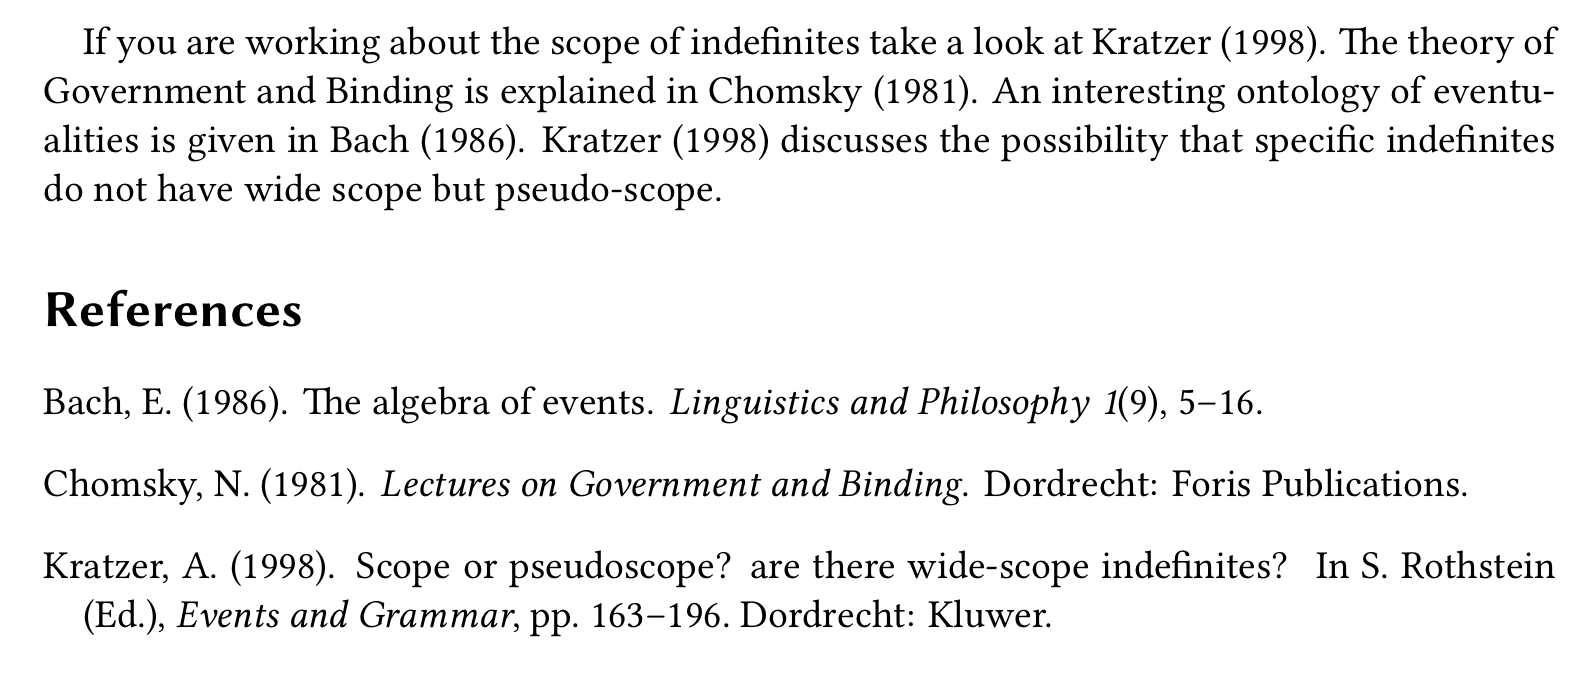
\includegraphics[width=.85\textwidth]{../../texfiles-beamer/tex-material/WissArb-latex/xelatex-bib-chicago-pdf}
\end{figure}

\end{frame}


%%%%%%%%%%%%%%%%%%%%%%%%%%%%%%%%%%
\begin{frame}[fragile]
\frametitle{Style: langsci-unified}


\begin{figure}
\centering
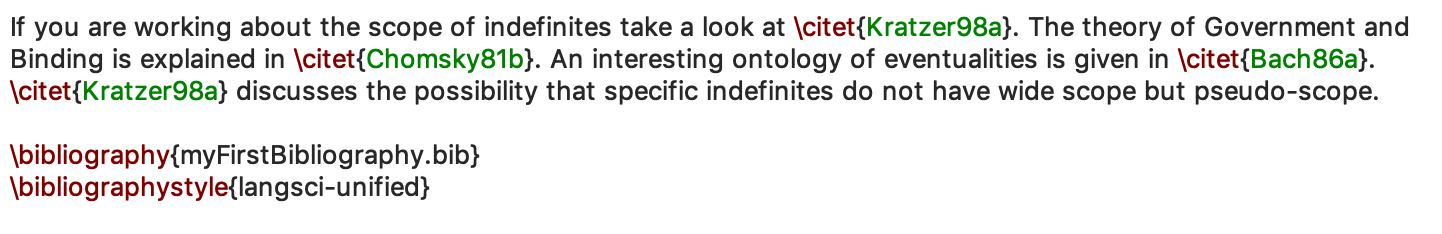
\includegraphics[width=.85\textwidth]{../../texfiles-beamer/tex-material/WissArb-latex/xelatex-bib-langsciunified}
\end{figure}

\begin{figure}
\centering
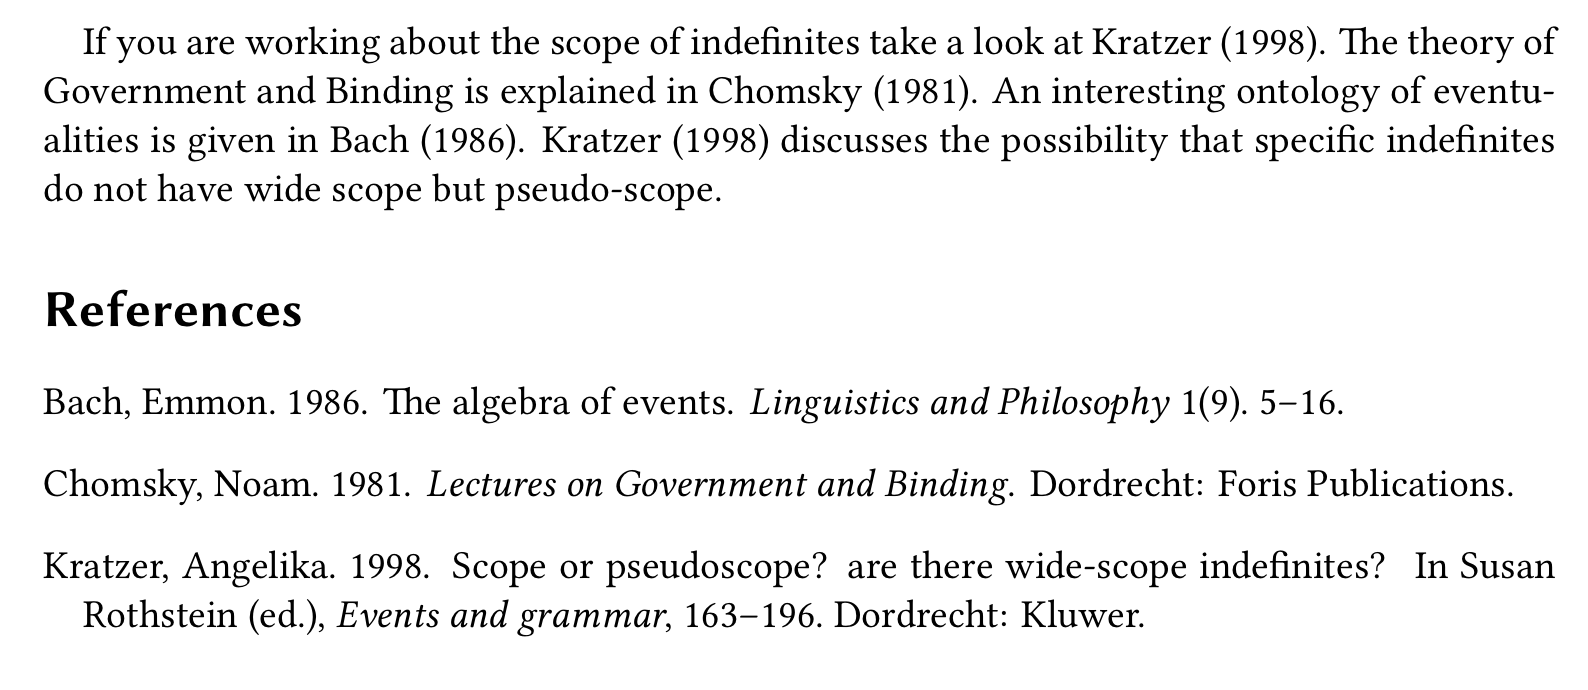
\includegraphics[width=.85\textwidth]{../../texfiles-beamer/tex-material/WissArb-latex/xelatex-bib-langsciunified-pdf}
\end{figure}

\end{frame}


%%%%%%%%%%%%%%%%%%%%%%%%%%%%%%%%%%%
%\begin{frame}[fragile]
%\frametitle{Stil: chicago auf Deutsch}
%
%\begin{itemize}	
%\item Eine Version des \ltxterm{chicago}-Stils für das Deutsche angepasst (\ltxterm{deChicagoMyP}) finden Sie im Moodlekurs. Speichern Sie die Datei \ltxterm{deChicagoMyP.bst} \textbf{in dem gleichen Ordner} wie Ihre \ltxterm{.tex}-Datei und verwenden Sie den Stil wie immer:
%\end{itemize}
%
%\begin{figure}
%\centering
%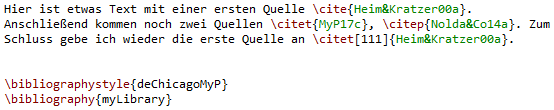
\includegraphics[width=.70\textwidth]{../../texfiles-beamer/tex-material/WissArb-latex/bib_deChicago_tex}
%\end{figure}
%
%\end{frame}
%
%
%%%%%%%%%%%%%%%%%%%%%%%%%%%%%%%%%%%
%\begin{frame}[fragile]
%\frametitle{Stil: deChicagoMyP}
%
%\begin{figure}
%\centering
%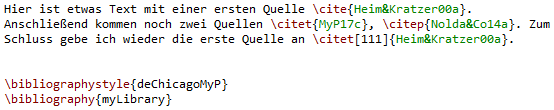
\includegraphics[width=.70\textwidth]{../../texfiles-beamer/tex-material/WissArb-latex/bib_deChicago_tex}
%\end{figure}
%
%\begin{figure}
%\centering
%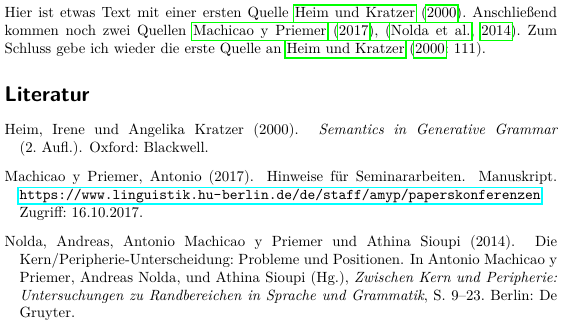
\includegraphics[width=.70\textwidth]{../../texfiles-beamer/tex-material/WissArb-latex/bib_deChicago_pdf}
%\end{figure}
%
%\end{frame}

%%%%%%%%%%%%%%%%%%%%%%%%%%%%%%%%%
\begin{frame}[fragile]
\frametitle{Exercise}


Go to \url{https://github.com/langsci/latex4linguists/blob/master/2-2.md}\\
and follow the instructions of \textbf{all blocks} in your \texttt{.tex} file.

%Download the PDF \alert{\texttt{myDocument-EX4.pdf}} and replicate it with the commands you have already learnt. Follow the instructions in the last section and install the packages.

\end{frame}


%%%%%%%%%%%%%%%%%%%%%%%%%%%%%%%%%%%
%%%%%%%%%%%%%%%%%%%%%%%%%%%%%%%%%%%
%\section{XY}
%%\frame{
%%\begin{multicols}{2}
%%\frametitle{~}
%%	\tableofcontents[currentsection]
%%\end{multicols}
%%}
%%%%%%%%%%%%%%%%%%%%%%%%%%%%%%%%%%%
%
%\begin{frame}{XY}
%
%\begin{itemize}
%	\item XY
%\end{itemize}
%
%\end{frame}


%%%%%%%%%%%%%%%%%%%%%%%%%%%%%%%%%%%%
%%%%%%%%%%%%%%%%%%%%%%%%%%%%%%%%%%%%
%\iftoggle{handout}{
%%% BEGIN handout true
%
%%%%%%%%%%%%%%%%%%%%%%%%%%%%%%%%%%%%
%	
%%Test Toggle ON
%
%}
%%% END handout true 
%%% BEGIN handout false
%{
%%%%%%%%%%%%%%%%%%%%%%%%%%%%%%%%%%%%
%
%% Test Toggle OFF
%
%}%% END handout false
%%%%%%%%%%%%%%%%%%%%%%%%%%%%%%%%%%%%